\section{Error Analysis}
\label{sec:error-analysis}




\paragraph{Overview.}
The main results show that agents often fail even after substantial retrieval and tool interaction, suggesting that the key bottleneck lies inside the trajectory rather than only in final-answer generation.
We therefore analyze failures in three stages:
\textbf{(1) Section~\ref{sec:error-planning-failures}} first studies how planning trajectories break in the default setting: agents often make partial progress, drift away from valid solution paths, and then fail to recover.
We further show that this drift is frequently not caused by the absence of useful retrieved tools, but by the model's failure to select or return to tools that would move the trajectory forward.
\textbf{(2) Section~\ref{sec:error-blocking}} then uses retrieval-time blocking as a controlled stress test of this selection and recovery weakness.
When a required tool is replaced by a corrupted alternative, the agent must detect that the current branch is unreliable and re-plan from remaining feasible paths; failures under blocking therefore reveal whether models can reject misleading or executable-looking bad evidence.
\textbf{(3) Section~\ref{sec:error-modelwise}} compares model-specific termination behaviors after navigation has already failed, showing how different model families expose the same underlying trajectory breakdown through distinct ending patterns. 


\subsection{Trajectory Drift and Tool-Selection Failures}
\label{sec:error-planning-failures}

To investigate planning failures in \bench{}, we annotate valid tool calls according to whether they advance a feasible solution path.
We define a tool call as a \textbf{\textit{progress call}} if it produces a new intermediate value needed by at least one valid tool-use path toward the final answer.
Otherwise, it is a \textbf{\textit{non-progress call}}.
This definition does not require the model to follow one fixed ground-truth path; it rewards any step that obtains useful intermediate evidence for completing the task.
Using this definition, we categorize failed trajectories as follows:
\begin{itemize}[topsep=2pt, partopsep=3pt, leftmargin=*, itemsep=-3pt]
\item \textbf{\textit{No Traction}}: the failed trajectory never makes a progress call, so the model obtains no useful intermediate evidence toward the final answer.
\item \textbf{\textit{Irrecoverable Drift}}: the model makes at least one progress call, then makes a non-progress call, and never makes progress again.
\item \textbf{\textit{Weak Recovery}}: the model makes progress again after a non-progress call, but still fails before reaching the correct answer.
\item \textbf{\textit{Format Error}}: the failure is caused by invalid or incompatible formatting (e.g., tool call or retrieval format) in the interaction process.
\end{itemize}
The first three categories describe where a failed trajectory breaks during solution-path execution, while \textit{Format Error} captures interface-level failures that we report separately from the main navigation analysis.

\begin{figure}[t]
\centering
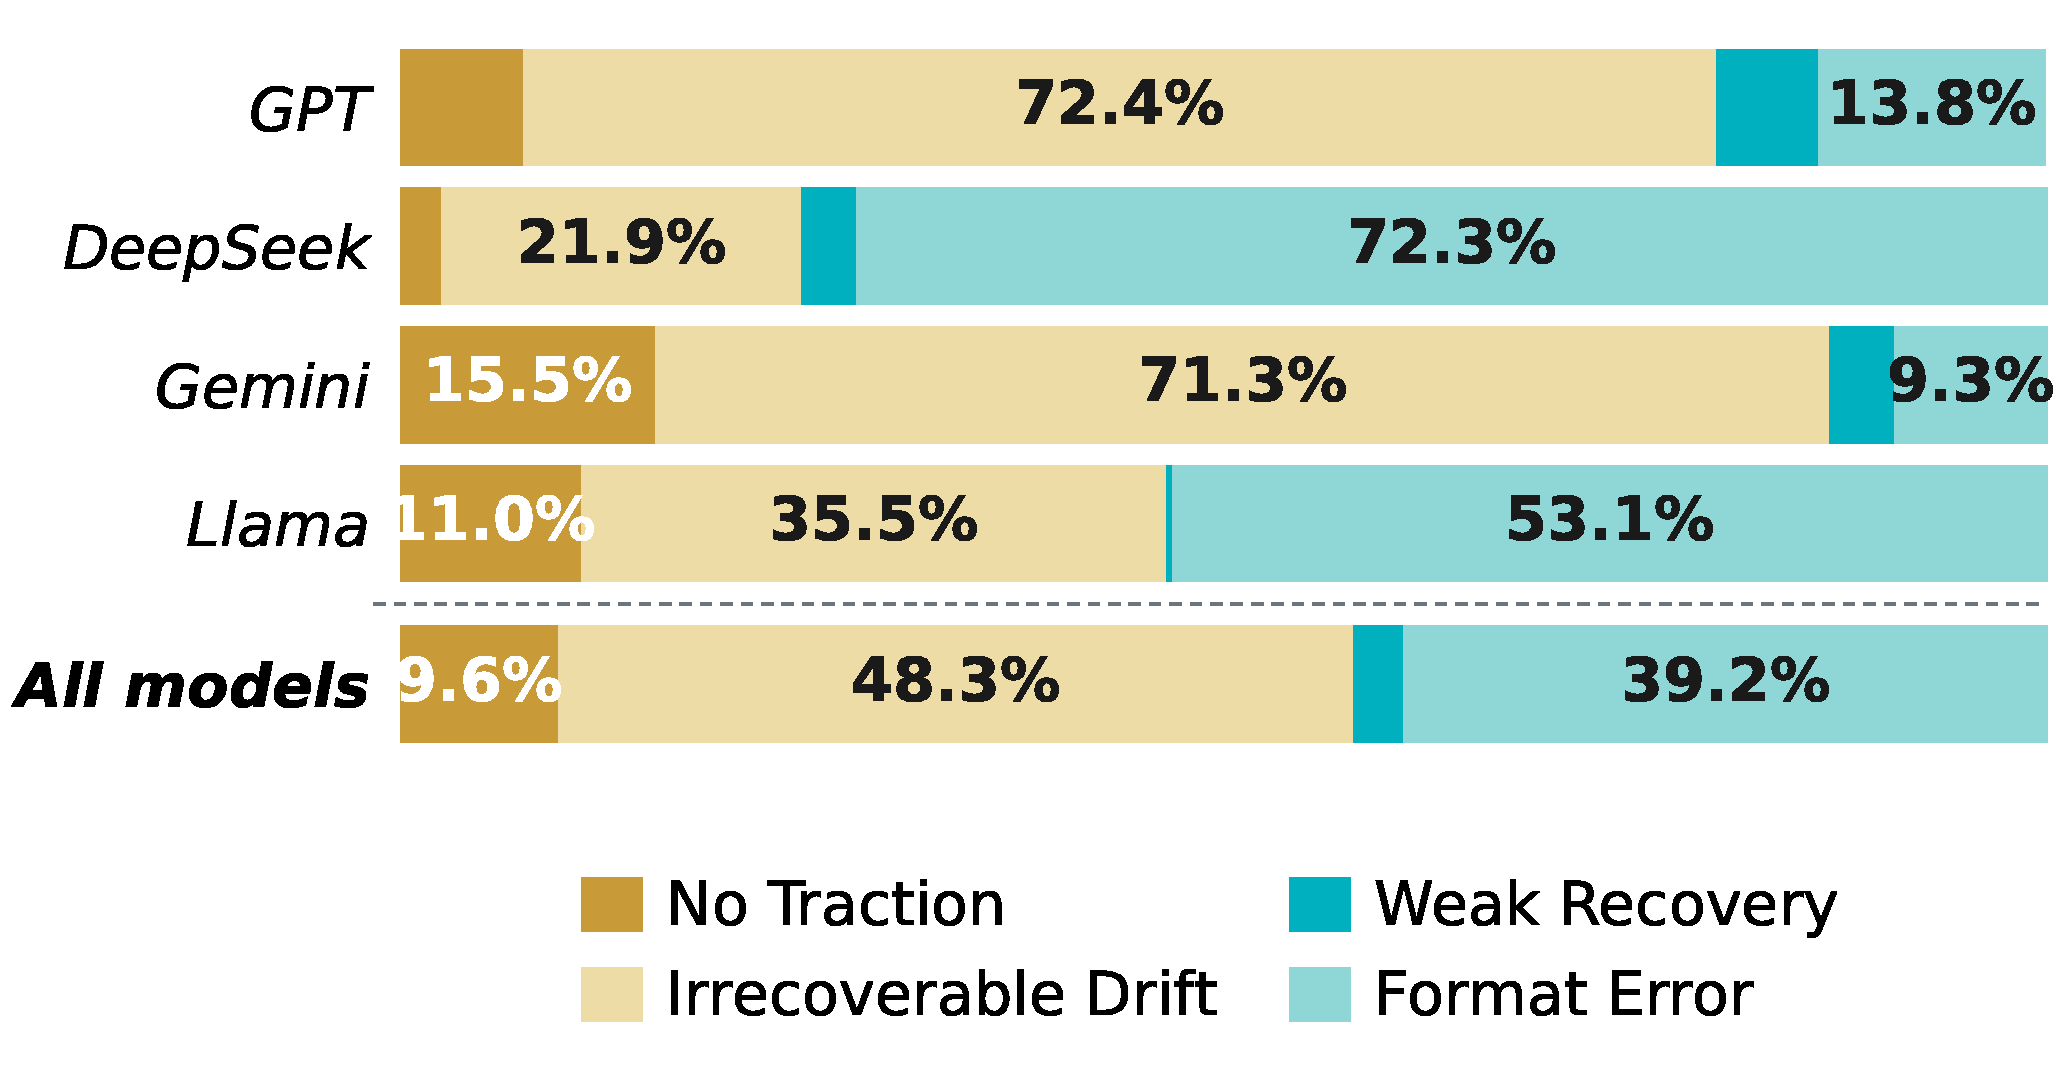
\includegraphics[width=1\linewidth]{Figures/mechanistic_navigation_breakdown_pdf.pdf}
\vspace{-0.2in}
\caption{
Trajectory Failure Category Distribution under the \textit{default} setting (\%). A tool call is counted as a progress call if it produces a new intermediate value required by at least one ground-truth tool-use path toward the final answer. We abbreviate \textit{GPT-5.4}, \textit{Gemini-3.5-Flash}, \textit{DeepSeek-V4-Flash}, and \textit{Llama-3.3-70B-Instruct} as \textit{GPT}, \textit{Gemini}, \textit{DeepSeek}, and \textit{Llama}.
}
\label{fig:mechanistic_navigation_breakdown}
\vspace{-0.12in}
\end{figure}

% \subsection{Definitions}
% \label{sec:mechanistic-error-definitions}

% \paragraph{Progress is defined by useful intermediate evidence.}
% We analyze failed trajectories by asking whether each successful tool call moves the agent closer to a valid solution.
% A tool call is a \emph{progress call} if it produces a new intermediate value that is needed by at least one valid tool-use path toward the final answer.
% Otherwise, it is a \emph{non-progress call}.
% This definition does not require the model to follow one fixed ground-truth path.
% Instead, it rewards any step that obtains useful intermediate evidence for completing the task.

% \begin{table*}[t]
% \centering
% \small
% \begin{tabular}{p{0.22\linewidth}p{0.70\linewidth}}
% \toprule
% \textbf{Category} & \textbf{Meaning} \
% \midrule
% \emph{No Traction} &
% The failed trajectory never makes a progress call. The model does not obtain any useful intermediate evidence toward the final answer. \

% \emph{Irrecoverable Drift} &
% The model makes at least one progress call, then makes a non-progress call, and never makes progress again. The trajectory initially moves toward a valid solution but later drifts away and does not recover. \

% \emph{Weak Recovery} &
% The model makes progress again after a non-progress call, but still fails before reaching the correct answer. The model partially recovers but does not complete the task. \

% \emph{Format Error} &
% The failure is caused by protocol, retrieval, label, tool-call, or resource-level errors, such as exceeding the maximum number of invalid tool calls. We report this separately because it reflects interface-following failure rather than planning failure. \
% \bottomrule
% \end{tabular}
% \caption{Compact taxonomy for mechanistic error analysis. The first three categories describe where a failed trajectory breaks during solution-path execution, while \emph{Format Error} captures interface-level failures outside the main navigation analysis.}
% \label{tab:mechanistic_error_taxonomy}
% \end{table*}

% \paragraph{\textbf{Solvability under blocking.}}
% Retrieval-time blocking replaces selected path-critical tools with blocked alternatives, but each blocked instance preserves at least one feasible tool-call path by construction.
% Therefore, failures under blocking should not be interpreted as cases where the task becomes unsolvable.
% Instead, they test whether the agent can detect that one plausible branch has become unavailable, unreliable, or misleading, and recover through another valid path.

% \subsection{Main Findings}
% \label{sec:mechanistic-error-findings}

\begin{takeaway}
Most failures occur after models have already obtained partially useful evidence, but then drift away from all ground-truth solution paths and rarely recover.
\end{takeaway}

\paragraph{Failures usually happen after partial progress.}
Figure~\ref{fig:mechanistic_navigation_breakdown} shows that models do not simply fail from the start; instead, they often make partial progress before drifting away from valid solution paths.
In the default setting, \textit{Irrecoverable Drift} is the largest planning failure category for \textit{GPT-5.4} and \textit{Gemini-3.5-Flash}, accounting for $72.4\%$ and $71.3\%$ of their reported failure categories, respectively, and remains the dominant category when aggregated across all four analyzed models.
This indicates that models often begin following a useful solution direction, but later take an off-path tool call that stops further progress.

\paragraph{Recovering after drift is difficult.}
The same figure shows that \textit{Weak Recovery} accounts for only $3.0\%$ of the reported default failure categories when aggregated across models.
This low recovery rate suggests that the main difficulty is not simply failing to find a useful tool-use direction.
Many failed trajectories make partial progress at first, but then a single non-progress step can push the agent away from the productive solution direction.
After such drift occurs, agents rarely repair the trajectory sufficiently to complete the task, suggesting that current agents still lack a stable adaptive re-planning mechanism for detecting and self-correcting unproductive directions.

\begin{takeaway}
Drift is often a tool-selection failure, not simply a retrieval failure.
\end{takeaway}

\paragraph{Useful alternatives are often already in the retrieved history.}
A natural explanation for such drift is that the agent may fail to retrieve any tool that can advance the current solution path.
Before failed-run \textit{non-progress calls}, the model had already retrieved at least one valid tool that could support progress toward the solution in $78.0\%$ of default cases and $71.1\%$ of block cases.
Thus, many wrong calls occur even though the model has already seen a solution-relevant alternative.
The bottleneck is therefore not only tool discovery, but also deciding which discovered tool should be used next.

\paragraph{Models over-select recently retrieved tools.}
The failed \textit{non-progress calls} also show a strong recency pattern in tool selection.
In both settings, most \textit{non-progress calls} use tools from recent retrieval windows, accounting for $74.1\%$ in the default setting and $63.6\%$ in the block setting.
However, when a clean tool that could make progress is available, it is often not recent: $44.7\%$ of default cases and $43.2\%$ of block cases involve such tools that were retrieved more than two retrieval windows earlier.
This contrast suggests that models tend to act on recently retrieved tools even when older tools would provide more useful progress toward the final answer.

\paragraph{Even when tools that could advance the task re-appear, agents still do not reliably recover.}
This failure cannot be reduced to memory loss alone.
After drift, a tool whose execution would be counted as a \textit{progress call} re-appears in the recent retrieval context in $42.5\%$ of default cases and $53.4\%$ of block cases.
In these cases, the issue is not that the useful tool only appeared in earlier retrieval history: it becomes available again after the trajectory has already drifted.
Yet the model still often fails to select it.
Recovery therefore requires more than retrieving additional tools or extending the interaction budget.
Agents need to retain useful candidates seen earlier and re-rank both previously seen and newly retrieved tools according to whether executing them would move the trajectory toward the final target.


\paragraph{Selection failure explains why broad exploration is not sufficient.}
This diagnosis also clarifies the gap between exploration and success observed in the main results.
Broad retrieval can expose useful intermediate information, but it does not guarantee that the model will exploit the right tool at the right time.
A model may retrieve many tools, or repeatedly search after drifting, while still failing to choose the progress-capable tool already available in its history.
The core navigation bottleneck is therefore the transition from discovery to useful execution.

\begin{figure}[t]
    \centering
    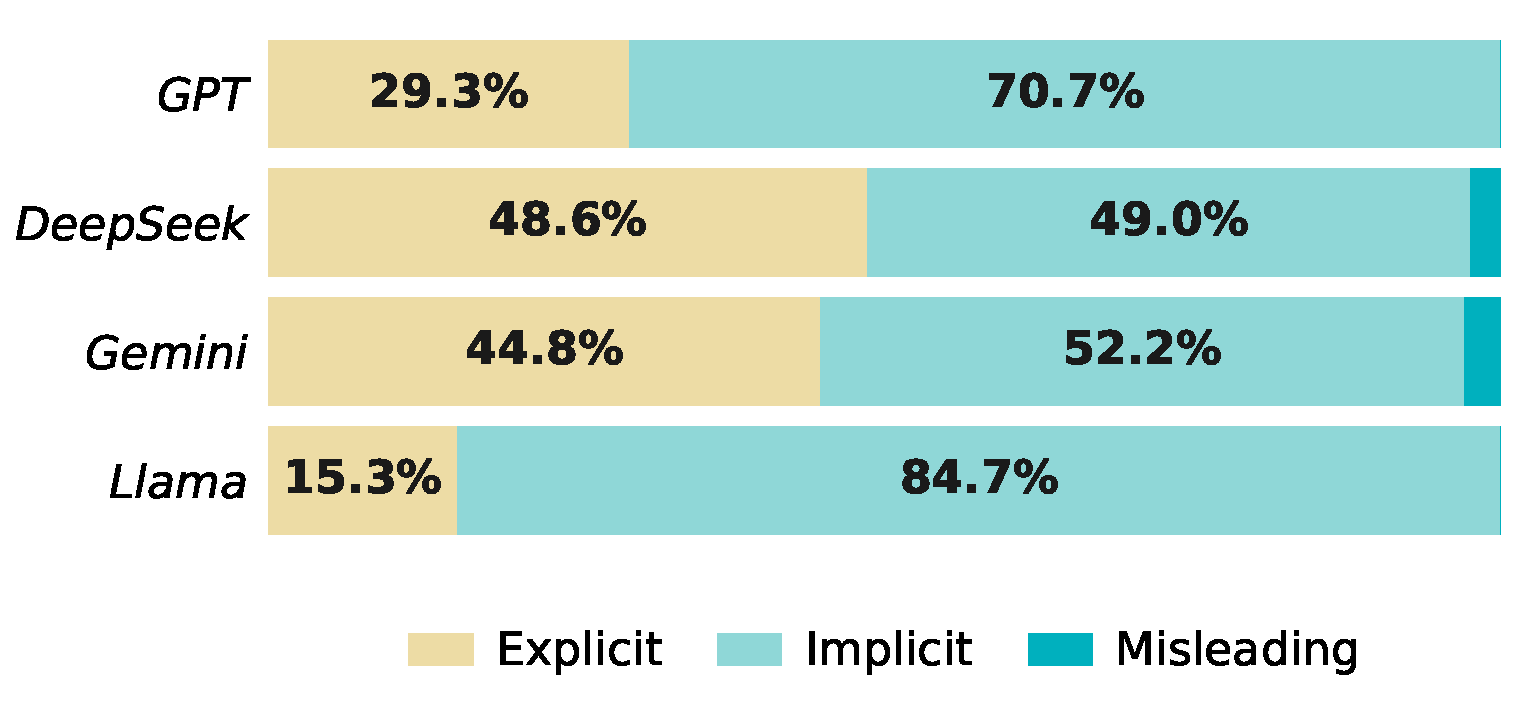
\includegraphics[width=1\linewidth]{Figures/noisy_tool_behavior_inner_bar.pdf}
    \vspace{-0.35in}
    \caption{Distribution of invoked block alternatives under \textit{mixed} blocking. For each model, the horizontal bar normalizes all invoked block alternatives to $100\%$. Colors indicate whether the invoked block alternative is an explicit failure, implicit failure, or semantic misleading tool. We abbreviate \textit{GPT-5.4}, \textit{Gemini-3.5-Flash}, \textit{DeepSeek-V4-Flash}, and \textit{Llama-3.3-70B-Instruct} as \textit{GPT}, \textit{Gemini}, \textit{DeepSeek}, and \textit{Llama}.}
    \label{fig:noisy_tool_type_mix}
    % \vspace{-0.2in}
\end{figure}



\subsection{Blocked-Alternative Misuse}
\label{sec:error-blocking}

% \paragraph{Blocking further exposes failures in tool selection and recovery.}
% The previous analysis shows that many failures arise even when useful tools have already been retrieved, because models do not reliably select or recall tools that would make useful progress.
% Retrieval-time blocking turns this weakness into a controlled stress test.
% When a required tool is replaced by a blocked alternative, the agent must recognize that the current branch is unreliable and recover through another feasible path.
% Since blocked instances remain solvable by construction, success requires not only finding tools, but also rejecting corrupted branches and re-planning from the remaining valid alternatives. \jy{Make this shorter, and link the to analysis part that have mentioned which type is damaging, and this time we are essentially using more fine-grained way to analyze it.}

The previous error analysis shows that many failures arise even when useful tools have already been retrieved, because models do not reliably select or recall tools that would make useful progress. Retrieval-time blocking turns this weakness into a controlled stress test. In Takeaway~\ref{tak:analysis-block-type-severity}, we have already shown that block types differ in severity, with silent failures causing especially large performance drops. Here, we move from aggregate performance to fine-grained tool-use behavior: when a required tool is replaced by a block alternative, success depends on whether the agent can detect the disrupted branch, avoid propagating corrupted observations, and re-plan through the remaining feasible paths.



% \paragraph{Blocked-alternative follow-up analysis.}
Figures~\ref{fig:noisy_tool_type_mix} and~\ref{fig:noisy_tool_followup_behavior} analyze agents' behavior after they invoke block alternatives returned under retrieval-time blocking.
Here, block alternatives refer to the additional tools inserted in place of blocked executable tools.
Figure~\ref{fig:noisy_tool_type_mix} shows which type of block alternative each model invokes.
Figure~\ref{fig:noisy_tool_followup_behavior} further shows how agents use the output of each invoked block alternative in later steps.
We categorize follow-up behavior into three cases:
\begin{itemize}[topsep=2pt, partopsep=3pt, leftmargin=*, itemsep=-3pt]
\item \textbf{\textit{Unused}}: the agent uses neither the tool's output information for later retrieval nor its returned value in a later tool call.
\item \textbf{\textit{Search Reused}}: the agent uses the tool's output information to retrieve further tools, but does not use its concrete returned value as an argument in a later tool call.
\item \textbf{\textit{Value Reused}}: the agent uses the tool's concrete returned value as an argument in a later tool call.
\end{itemize}
This distinction separates two ways in which a block alternative can affect later planning.
A model may continue from the block alternative's declared output information without trusting the returned value, or it may directly propagate the returned value into later tool calls.



\begin{takeaway}
Models can reject superficial distractors but struggle with executable-looking failures, especially silent ones with superficially plausible outputs.
\end{takeaway}


\paragraph{Semantically misleading tools are usually not the main issue.}
Across models, semantic misleading tools account for at most $3\%$ of invoked block alternatives, and are never selected by \textit{GPT-5.4} or \textit{Llama-3.3-70B-Instruct}.
This suggests that current models can often use tool names and descriptions to reject alternatives whose functions are only superficially related to the current need.
The more difficult cases are block alternatives that look compatible with the current schema or return concrete values that appear usable.

\paragraph{Explicit failures stop direct value propagation but not follow-up search from the failed tool.}
After invoking explicit-failure block alternatives, agents never use the returned error message as an argument in later tool calls.
This shows that explicit error signals are effective at preventing direct propagation of obviously invalid values.
However, explicit failures do not always stop the agent from searching for follow-up tools from the failed call.
Agents may still use the failed tool's declared output information to retrieve downstream tools, even though the concrete execution did not produce a valid value.
Thus, explicit errors make the failed branch visible, but they also expose a remaining challenge: the model must still abandon that branch and re-plan through another feasible path.

\begin{figure}[t]
    \centering
    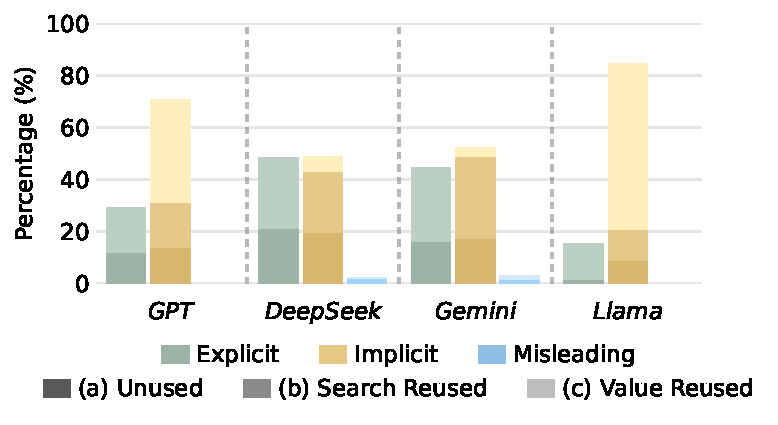
\includegraphics[width=1\linewidth]{Figures/noisy_tool_behavior_outer_bar_vertical.pdf}
    \vspace{-0.35in}
    \caption{Follow-up behavior after agents invoke block alternatives under \textit{mixed} blocking. Each colomn corresponds to one model and one block type. The row length shows the ratio of all invoked block alternatives for that model, and colored segments denote \textit{Unused}, \textit{Search Reused}, and \textit{Value Reused}. \textit{GPT} denotes \textit{GPT-5.4}, \textit{Gemini} denotes \textit{Gemini-3.5-Flash}, \textit{DeepSeek} denotes \textit{DeepSeek-V4-Flash}, and \textit{Llama} denotes \textit{Llama-3.3-70B-Instruct}.}
    \label{fig:noisy_tool_followup_behavior}
    \vspace{-0.2in}
\end{figure}

\paragraph{Implicit failures turn drift into value contamination.}
Implicit failures are more damaging because they return superficially plausible concrete values instead of explicit error messages.
For \textit{GPT-5.4} and \textit{Llama-3.3-70B-Instruct}, \textit{Value Reused} accounts for $55.9\%$ and $75.5\%$ of implicit-failure follow-ups, respectively; aggregated across models, implicit failures lead to \textit{Value Reused} in $42.2\%$ of cases, compared with $0\%$ for explicit failures.
This means that silent failures do not merely stop progress.
They inject invalid values that the agent treats as grounded evidence for later tool calls.
Once these values enter the trajectory, subsequent calls may look procedurally valid while moving the agent further away from any valid solution.

% \paragraph{Silent failures hide the need to backtrack.}
% The difference between explicit and implicit failures explains why corrupted tool environments amplify the navigation weakness identified above.
% When a tool returns an explicit error, the model receives a visible signal that the current branch is broken, even if it does not always recover correctly.
% When a tool returns a plausible but wrong value, the model may not realize that recovery is needed at all.
% The agent then continues executing from a corrupted state, making the failure harder to detect, contain, and repair.
% Thus, blocker-induced degradation is not only caused by having fewer feasible paths; it is also caused by the model's inability to distinguish reliable intermediate evidence from silent failure outputs.

\subsection{Model-Specific Failure Patterns}
\label{sec:error-modelwise}

% \paragraph{\textbf{Termination behavior is separate from the navigation failure itself.}}
% The previous findings describe where the trajectory breaks and why recovery is difficult.
% We next ask how models behave after their trajectory is no longer grounded in a valid solution path.
% We treat these final behaviors as termination policies rather than primary failure mechanisms, because the same trajectory-level failure can end in different surface outputs.
% A model may explicitly surrender, return a wrong value obtained from an off-path tool, confabulate an unsupported value, or continue searching until the interaction budget is exhausted.

% % \begin{table*}[t]
% % \centering
% % \small
% % \setlength{\tabcolsep}{5pt}
% % \begin{tabular}{lccccc}
% % \toprule
% % \textbf{Model}
% % & \textbf{Failed runs}
% % & \textbf{No Traction}
% % & \textbf{Irrecoverable Drift}
% % & \textbf{Weak Recovery}
% % & \textbf{Interaction Breakdown} \\
% % \midrule
% % \textit{GPT-5.4} & 152 & 7.2 & 69.1 & 5.9 & 13.2 \\
% % \textit{DeepSeek-V4-Flash} & 120 & 2.5 & 21.7 & 3.3 & 71.7 \\
% % \textit{Gemini-3.5-Flash} & 153 & 13.1 & 60.1 & 3.3 & 7.8 \\
% % \textit{Llama-3.3-70B-Instruct} & 265 & 10.9 & 35.1 & 0.4 & 52.5 \\
% % \midrule
% % \textbf{All models} & 690 & 9.1 & 45.8 & 2.8 & 37.2 \\
% % \bottomrule
% % \end{tabular}
% % \caption{Default-setting trajectory failure categories (\% of failed runs). A successful call is counted as progress if it produces a new intermediate value needed by at least one valid tool-use path toward the final answer.}
% % \label{tab:mechanistic_navigation_breakdown}
% % \end{table*}

% \begin{table*}[t]
% \centering
% \small
% \setlength{\tabcolsep}{5pt}
% \resizebox{\linewidth}{!}{
% \begin{tabular}{llcccccc}
% \toprule
% \multirow{2}{*}{\textbf{Model}}
% & \multirow{2}{*}{\shortstack{\textbf{Dominant}\\\textbf{Ending}}}
% & \multicolumn{2}{c}{\textbf{\# Non-interaction Failures}}
% & \multicolumn{2}{c}{\textbf{Dominant Ending Ratio (\%)}}
% & \multicolumn{2}{c}{\textbf{Failure-only S/C Ratio}} \\
% \cmidrule(lr){3-4}
% \cmidrule(lr){5-6}
% \cmidrule(lr){7-8}
% & &
% \textbf{Default} & \textbf{Blocker} & \textbf{Default} & \textbf{Blocker} & \textbf{Default} & \textbf{Blocker} \\
% \midrule
% \textit{GPT-5.4}
% & Surrender & 132 & 139 & 77.3 & 80.6 & 4.5 & 4.2 \\
% \textit{DeepSeek-V4-Flash}
% & Wrong tool value & 34 & 44 & 58.8 & 65.9 & 6.1 & 4.6 \\
% \textit{Gemini-3.5-Flash}
% & Search exhaustion & 141 & 154 & 90.8 & 85.1 & 29.1 & 18.3 \\
% \textit{Llama-3.3-70B}
% & Wrong tool value & 126 & 106 & 81.7 & 71.7 & 2.1 & 2.0 \\
% \bottomrule
% \end{tabular}
% }
% \caption{
% The most frequent ending type for each model after planning failures.
% \emph{\# Non-interaction Failures} is the number of failures after excluding interaction breakdowns in the corresponding setting.
% \emph{Dominant Ending Ratio} is the share of those failures that end with the behavior named in the second column.
% \emph{Failure-only S/C Ratio} is the average S/C Ratio computed only over the non-interaction failure traces.
% \jy{check this table}
% }
% \label{tab:mechanistic_termination_behavior}
% \end{table*}

% \paragraph{Termination behavior is separate from the navigation failure itself.}
The previous findings describe where the trajectory breaks and why recovery is difficult.
We next ask how models behave after their trajectory is no longer grounded in a valid solution path.
We treat these final behaviors as termination policies rather than primary failure mechanisms, because the same trajectory-level failure can end in different surface outputs.
We define three dominant ending types:
\begin{itemize}[topsep=2pt, partopsep=3pt, leftmargin=*, itemsep=-3pt]
\item \textbf{\textit{Surrender}}: the final response explicitly states that the model cannot determine, verify, or provide the requested answer.
\item \textbf{\textit{Wrong tool value}}: the final response gives an incorrect answer that is not supported by any tool output relevant to the target query. The value may be fabricated or guessed, or it may be copied from another tool call whose output does not answer the requested query.
\item \textbf{\textit{Search exhaustion}}: the trajectory ends without a grounded answer after repeated retrieval/search actions fail to produce a decisive progress-making tool call.
\end{itemize}
% The \textit{dominant ending} denotes the most frequent ending type for each model.

\begin{takeaway}
After navigation failure, models expose different termination policies: GPT surrenders, DeepSeek and Llama commit wrong tool values, and Gemini keeps searching.
\end{takeaway}

\paragraph{GPT often surrenders despite the existence of valid solution paths.}
Among default non-interaction failures, \textit{GPT-5.4} ends $77.3\%$ with an explicit surrender statement, despite the prompt explicitly stating that each task is solvable, as shown in Figure~\ref{fig:inference-prompt}. Under the block setting, this rate further rises to $80.6\%$. These terminations therefore do not indicate genuinely unsolvable tasks: each blocked instance preserves at least one feasible solution path by construction. Rather, they suggest that \textit{GPT-5.4} often stops once its current branch no longer appears useful, instead of abandoning that branch and recovering through another valid path. Although this behavior is conservative in that the model usually avoids hallucinating an answer, it still reflects a failure of adaptive recovery in a solvable environment.

\paragraph{DeepSeek and Llama more often commit hallucinated values.}
\textit{DeepSeek-V4-Flash} commits wrong tool-returned values in $58.8\%$ of default failures and $65.9\%$ of block failures.
\textit{Llama-3.3-70B-Instruct} shows this pattern even more strongly, committing wrong tool values in $81.7\%$ of default failures and $71.7\%$ of block failures.
Compared with explicit refusal or surrender, this represents a more severe failure mode: the model still produces a final answer even when the trajectory has drifted away from any valid solution path. 
In such cases, it may rely on unsupported evidence, fabricate a value, or reuse an intermediate result from an irrelevant tool call as if it answered the target query.


\paragraph{Gemini keeps searching without converting search into progress.}
\textit{Gemini-3.5-Flash} ends $90.8\%$ of default failures and $85.1\%$ of block failures through search exhaustion.
Its S/C ratio averaged on the failed instances is also much larger than the other analyzed models, reaching $29.1$ in the default setting and $18.3$ under blocking.
This suggests that \textit{Gemini-3.5-Flash} mainly fails not by premature commitment, but by searching without making decisive progress.

% \paragraph{These termination policies are stable failure fingerprints.}
\paragraph{These model-specific failure fingerprints are stable across settings.}
The trajectory-level analysis shows that these model-specific patterns are largely stable across settings.
Across the tested blocking settings, the dominant failure pattern remains unchanged for \textit{DeepSeek-V4-Flash}, \textit{Gemini-3.5-Flash}, and \textit{Llama-3.3-70B-Instruct}, and also holds for \textit{GPT-5.4} in most settings.
This indicates that blocking, path length, feedback, and other interventions mostly change how often each model fails, rather than replacing its characteristic failure policy.
The resulting picture is therefore hierarchical: models first fail through weak solution-path execution and recovery, corrupted tools then amplify this weakness through uncontained failure branches, and each model finally exposes the broken trajectory through its own termination bias.

% \subsection{Implications}
% \label{sec:mechanistic-error-implications}

% \paragraph{\textbf{The resulting picture is hierarchical.}}
% At the trajectory level, models fail because they select non-progress tools and rarely recover after drift.
% At the blocker level, corrupted alternatives amplify this weakness by making the agent decide whether a branch is still trustworthy.
% At the model level, the same broken trajectory appears through different termination policies: surrender, wrong-value commitment, or continued search.
% Together, Tables~\ref{tab:mechanistic_navigation_breakdown}--\ref{tab:mechanistic_cross_setting_drift} support a single account: tool-use failures are governed by weak solution-path execution, weak failure containment, and model-specific stopping policies.

% \paragraph{\textbf{Better benchmark performance requires progress-aware tool selection.}}
% Table~\ref{tab:mechanistic_search_opportunity} shows that progress-capable tools are often already present in the retrieved history when the model makes a non-progress call.
% This implies that simply increasing retrieval volume or turn budget is unlikely to solve the dominant failure mode.
% Future agents should explicitly track whether each tool call advances toward the target, preserve useful earlier candidates, and re-rank tools by whether they help complete the remaining solution path.

% \paragraph{\textbf{Robust agents must reject corrupted intermediate evidence.}}
% Figures~\ref{fig:noisy_tool_type_mix} and~\ref{fig:noisy_tool_followup_behavior} show that the most harmful blocked alternatives are not necessarily those with visibly mismatched functionality.
% Instead, implicit failures are dangerous because they return plausible values that can be reused in later calls.
% This suggests that adaptive agents need mechanisms for validating intermediate values, detecting unreliable branches, and backtracking when a previously plausible tool-use path becomes untrustworthy.

% \paragraph{\textbf{Model-specific termination biases require different interventions.}}
% Table~\ref{tab:mechanistic_termination_behavior} shows that \textit{GPT-5.4} often surrenders despite remaining feasible paths, \textit{DeepSeek-V4-Flash} and \textit{Llama-3.3-70B-Instruct} often commit wrong tool-returned values, and \textit{Gemini-3.5-Flash} often searches until exhaustion.
% These patterns suggest that the same solution-path failure may require different fixes across models.
% For GPT-like models, the key issue is recovering rather than surrendering in solvable tasks.
% For DeepSeek- and Llama-like models, the key issue is preventing off-path values from being over-trusted.
% For Gemini-like models, the key issue is converting continued search into progress-making execution.
